The scope of this work includes development and demonstration of
various methods and tools to leverage Cyclus' existing
capabilities to model and simulate real-world nuclear fuel cycle
transition scenarios involving advanced reactor technologies.


\section{Background}
Increasing climate change concerns have directed attention
to nuclear energy, which produces reliable baseload energy
with negligible CO$_2$ emission. To reduce CO$_2$ emissions,
the world will have to reduce fossil fuel power plants.
Also, the world energy demand is expected to increase
(28\% growth between 2015 and 2040 \cite{conti_international_2016}).
Given the two circumstances,
nuclear power is expected to play a crucial role in the world energy portfolio.

However, concerns of the accumulating \gls{UNF} inventory,
safety of the current reactor fleet, and the availability of
uranium resources create a negative public perception of
nuclear energy and its sustainability.

Advanced fuel cycles that recycle nuclear fuel 
provide an opportunity for solving those concerns while
meeting energy demand. Towards the effort to transition
into advanced fuel cycles, the \gls{ANS} \gls{FCWMD} has identified
three grand challenges \cite{huff_message_2017}, listed below. The grand
challenges are technical goals that need to be resolved by
2030 in order to help solve some of the economic, sociological,
or political issues that the nuclear society face \cite{american_nuclear_society_ans_2017}.

\begin{enumerate}
	\item Establish used nuclear fuel recycling associated with the
	``most promising'' fuel cycles that are economically competitive
	with current electricity production.
	\item Leverage the findings of the U.S. \gls{DOE}'s Evaluation
	and Screening Study to reconsider the U.S. approach to the whole
	nuclear fuel cycle, and publicly establish the ``most promising''
	nuclear fuel cycles and address some of the stretched ``truths''
	about some fuel cycles.
	\item Establish a logical incremental timeline toward a pilot
	and full-scale recycling facility for current reactors, and
	transition to future reactors from the ``most promising'' fuel cycles.
\end{enumerate}

The three grand challenges can be summarized as a need to
identify and plan for a ``most promising'' fuel cycle, while
accurately calculating its impacts. 
A simulation tool capable of accurately calculating the metrics
of a fuel cycle transition scenario is essential for solving these challenges.

This work will demonstrate capabilities of a system-level
analysis tool, Cyclus. The modeling capabilities of Cyclus 
will aid in the effort of solving
the grand challenges mentioned above.

\subsection{The nuclear fuel cycle}
The nuclear fuel cycle is the complete nuclear energy
system from mining to disposal \cite{tsoulfanidis_nuclear_2013}.
A common goal of
a \gls{NFC} is to produce power economically, while minimizing
waste and natural resource used. Other specialized goals of \gls{NFC}s may involve
weapons material production or repository burden reduction through transmutation.
The discharge \gls{UNF} from the reactors is eventually sent back to facilities for
either recycling or disposal.

In 2011, the \gls{DOE} commissioned a report based on the national priorities
in order to plan the U.S. nuclear future.
The report by Wigeland et al. identified potential fuel cycle groups and compared them
to find the most `promising' fuel cycle \cite{wigeland_nuclear_2014}.
The objective of the evaluation was to provide information about the
potential benefits and challenges of nuclear fuel cycle options, in order to
guide \gls{DOE} \gls{FCRD} program.
This study identified 40 fuel cycle groups, categorized by the extent of recycling
(no recycle, limited recycle, and continuous recycle), fuel composition
(e.g. thorium-U233, uranium-plutonium), and the type of reactors (fast/thermal critical
reactors, sub-critical \gls{EDS}).

Fuel Cycles can be mainly categorized by their treatment of \gls{UNF}. A
fuel cycle that disposes all \gls{UNF} generated is a once-through fuel cycle.
If the \gls{UNF} is reprocessed, a fuel cycle is categorized either as a
closed fuel cycle, or a fuel cycle with limited recycling, depending on
the cycles fuel might undergo transmutation. 

\subsubsection{Once-through fuel cycle}

In a once-through cycle, nuclear fuel is used once and then sent to
storage without further reprocessing \cite{tsoulfanidis_nuclear_2013}.
This cycle is often called the open fuel cycle, and is the current cycle for
most nations with nuclear energy (e.g. U.S., Korea, Finland, Sweden).

This fuel cycle begins with mining of uranium or thorium ore, which is extracted from the
ground. The mined ore is milled to form yellowcake ($U_3O_8$).
The yellowcake is then either converted to $UF_6$ and enriched, or converted
to $UO_2$ directly. This is because some reactor designs (e.g. \gls{CANDU} designs\cite{torgerson_candu_2006})
can operate with natural uranium, while others (e.g. \glspl{LWR}) need
higher-than-natural levels of uranium-235. The processed $UO_2$ is
then fabricated to pellets and loaded into fuel assemblies.

Once the fuel is depleted in the reactor, it is put in on-site pools to cool down.
After cooling, the \gls{UNF}
is stored in dry casks as interim storage, destined to be sent to a geologic repository
for permanent disposal.

\subsubsection{Closed fuel cycle}
In a closed fuel cycle, the \gls{UNF} is recycled to be reused
in a nuclear reactor. Recycling has two major
benefits: increased fuel utilization and reduction of repository
burden.

A typical composition of \gls{UNF} discharged from an \gls{LWR}
is approximately 95\% uranium, 0.9\% plutonium, 0.1\%
minor actinides, and 4\% fission products \cite{feiveson_spent_2011}.
The uranium, plutonium, and minor actinides have the capability
to produce power through fission. Thus, every group except the
fission products can be separated to create new fuel for other reactors.

Additionally, repository capacity is constrained mostly by decay heat
load and radioactivity, meaning that removal of the high-activity
isotopes leads to a more efficient utilization of the repository
capacity. Short-lived fission products (e.g. cesium, strontium) contribute
to significant heat and radioactivity in the first 100 years of \gls{UNF} disposal,
and long-lived minor actinides (americium, plutonium),
contribute to longer-term heat and radioactivity \cite{wigeland_separations_2006},
as shown in figure \ref{fig:decay_heat}.

\begin{figure}[htbp!]
	\begin{center}
		\hspace*{-1.5cm}
		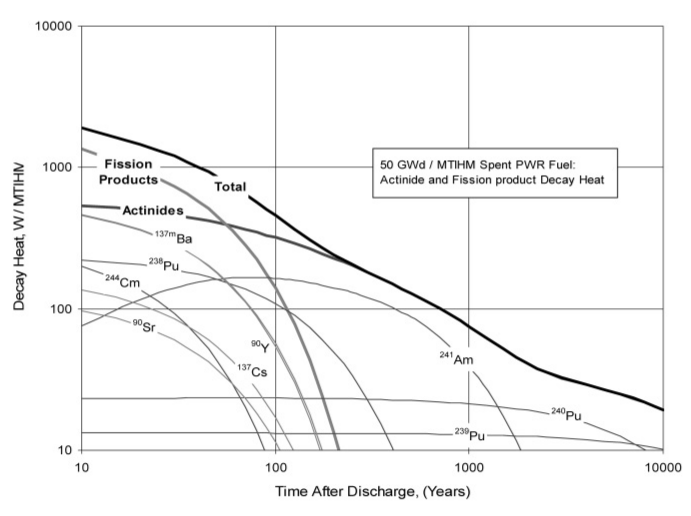
\includegraphics[scale=0.6]{./images/decay_heat.png}
	\end{center}
	\caption{Decay heat contributions in \gls{UNF} from a \gls{PWR} irradiated
		to 50 GWd/MTHM. Reproduced from Wigeland, 2006 \cite{wigeland_separations_2006}.}
	\label{fig:decay_heat}
\end{figure}


There are two major reprocessing technologies:
methods that use low-temperature chemical separation
using organic solvents (e.g. PUREX \cite{baumgaertner_purex_1976}), and
methods that use high-temperature molten salts and metals, like pyroprocessing
\cite{laidler_development_1997}. These methods separate the \gls{UNF}
into different streams, which are then sent to either a \gls{HLW} repository
(fission products) or an appropriate fuel fabrication facility (plutonium).

Different closed fuel cycles use different elemental groups for recycled
fuel fabrication. For example, the PUREX process is used in La Hague in France
\cite{schneider_spent_2008}, THORP in the U.K \cite{riley_technology_1998},
Mayak in Russia, and Rokkasho in Japan to separated plutonium and uranium
\cite{birkett_recent_2005}. The plutonium is mixed with either depleted
uranium (tails) or reprocessed uranium to produce \gls{MOX}.

Closed fuel cycles
generally involve fast-spectrum reactors to control TRU inventory.
A fast-spectrum reactor can be designed to either burn (reduce TRU),
breed (produce more TRU), or break-even (maintain TRU amount).
Selection of the fast-spectrum reactor design depends on the
goal of the deploying institution.


\subsubsection{Fuel cycle with limited recycling}
Fuel cycle with limited recycling is defined by the recycling of \gls{UNF}
for a limited number of times. 
The goals for recycling the irradiated fuel include
reusing the separated material in a nuclear reactor and 
separating long-lived highly radioactive elements
for repository burden reduction \cite{wigeland_nuclear_2014}.
The difference
between limited recycling and `closed' fuel cycles (continuous
recycling) is the number of cycles fuel might undergo transmutation.
In `closed' fuel cycle, the fuel undergoes many to an infinite number
of cycles, through constant reprocessing.


\subsection{Fuel cycle transition scenarios}
In a fuel cycle transition, an initial fleet of technology and corresponding
fuel cycle strategies dynamically evolve into a different final state \cite{oecd_nuclear_2009}.
In this work, I focus on the transition from
once-through fuel cycles to closed fuel
cycles through the progressive replacement of previous technology
(i.e. \glspl{LWR}) with an advanced technology (i.e. reprocessing
and fast-spectrum reactors). Other transition scenarios include
a general transition into a different fuel cycle (evaluation group
defined by Wigeland et al.), to a mixture of fuel cycles, or
a complete nuclear energy phaseout.

In this work, I analyze the material feasibility of fuel
cycle transition scenarios, which is characterized by whether
all nuclear reactors received fuel on time.

The fuel demand is determined by two factors - nuclear energy demand
and the nation's fuel cycle strategy.
The nuclear energy demand determines the construction
and operation
schedule of new reactors, and the fuel demand is
calculated accordingly.
Fuel cycle strategies determine the isotopic
requirements of the fuel cycle transition scenario. For example,
if the transition drives toward a U-Pu \gls{MOX} fuel cycle,
plutonium inventory dominates the timescale and feasibility of transition.

Once the expected fuel demand is calculated,
the initial condition - current fissile material inventory
and number of reactors (and their remaining lifetimes) - determines
the material feasibility and timescale of a transition scenario.
If a transition scenario is infeasible (i.e. fissile source is lacking) or delayed,
the transition can be `loosened', by delaying deployment
of advanced reactors. The energy demand can instead be met by additional
deployment of previous reactor technology (e.g. \glspl{LWR}),
thereby increasing transition timescale but reducing the
intensity of fissile material demand.

Since fuel cycles involve multiple facilities,
transition scenario analyses require
dynamic tracking of materials and facilities.
The dynamic tracking will calculate available nuclear material
inventory as well as the demand for the nuclear
material.

\subsection{Real-world fuel cycle simulation}
Real-world fuel cycle simulation captures the non-uniformity of
reactor facilities in the real world. Most work on fuel cycle
simulation assumes a uniform fleet of reactors with identical
parameters, such as core size and power capacity. This simplification
does not reflect the current state of nuclear operation, in which
reactors vary in power capacity and core size, leading
to errors in \gls{UNF} inventory and power demand calculations.
Capturing the real-world nuclear fleet requires discrete
modeling of facilities, with unique parameters for each facility
as well as discrete material and facility event (e.g. refuel outage,
decommission) modeling.


\section{Objectives}

This thesis demonstrates and extends the real-world \gls{NFC} transition
scenario modeling capabilities in Cyclus. 
The goal of this thesis to
develop tools that leverage Cyclus' modularity to
add capabilities required for modeling real-world
fuel cycle transition scenarios. The added capabilities are then
demonstrated through \gls{NFC} transition scenarios relevant to France and the United
States.

\section{Motivation}

There are two major motivations for accurately simulating
real-world \gls{NFC} transition scenarios.
First, \gls{NFC} transitions require strategized reactor
and fuel cycle deployment to meet fuel demand for advanced systems.
A simulation tool must be able to calculate the material
and facility throughput requirements of the transition scenario.
Second, \gls{NFC} transition scenarios need to optimize
existing investment and technology. For example, with an \gls{NFCS},
analysts can determine the best reactor technology
to leverage current \gls{LWR} \gls{UNF} inventory in a nation.



\section{Methods}
This thesis accomplishes the objective in three steps. 
First, a benchmark showed good agreement with other
fuel cycle simulation tools. \footnote{These results have been
submitted for publication in Annals of Nuclear Energy.}
Second, I identified and developed the tools and methods necessary
for modeling and simulating real-world transition scenarios.
Finally, I constructed and ran fuel cycle transition scenarios
relevant to France and the United States to demonstrate
and verify the capability.

\subsection{Benchmark study}
A previous study by Feng et al. \cite{feng_standardized_2016} validates existing 
\glspl{NFCS} in a fuel cycle transition scenario, in which an \gls{LWR} fleet
transitions into an \gls{SFR} fleet with continuous reprocessing. This 
study compares four well-known \glspl{NFCS}
DYMOND \cite{yacout_modeling_2005},
VISION \cite{jacobson_verifiable_2010},
ORION \cite{gregg_analysis_2012}, and
MARKAL \cite{shay_epa_2006}. The results from each code were
compared to a set of `model solutions' that were generated
from a spreadsheet for various metrics (e.g. fuel loading
in reactor, \gls{UNF} inventory). I reproduced the transition
scenario in Cyclus, and compare the Cyclus results with those
from the model solutions.

\subsection{Tool development}
In order to model real-world transition into an advanced
fuel cycle, I developed two major tools. First, I developed a python package \texttt{cyclus-input-gen},
which includes the submodule \texttt{from\_pris}
that automates extraction from the curated \gls{IAEA} \gls{PRIS} database
\cite{iaea_nuclear_2018}. Second, I developed \texttt{SaltProc\_Reactor}that models \glspl{MSR}
in Cyclus using a database generated from a high-fidelity \gls{MSR} depletion calculation.

\subsection{Real-world fuel cycle transition scenario simulation}
I constructed the fuel cycle transition scenario for France and the United States.
I made different assumptions for the two scenarios to account for each nation's different goals,
initial conditions (i.e. currently existing fleet, \gls{UNF} inventory), and their potential reactor
technology. I used \texttt{from\_pris} to construct the initial Cyclus input file,
followed by iterations to account for new reactor deployment. The workflow driving the analyses is shown in diagram \ref{diag:workflow}.


\begin{figure}
        \centering
\begin{tikzpicture}[node distance=1.5cm]
\node (database) [object] {Database (\texttt{.csv})};
\node (script) [process, below of=database] {Input Generation Module (\texttt{from\_pris})};
\node (input) [object, below of=script] {\Cyclus Input File (\texttt{.xml})};
\node (cyclus) [process, below of=input]{\Cyclus};
\node (output) [object, below of=cyclus]{\texttt{Output File (\texttt{.Sqlite})}};
\node (script2) [process, below of=output]{Analysis Script (\texttt{analysis.py})};

\draw [arrow] (database) -- (script); 
\draw [arrow] (script) -- (input); 
\draw [arrow] (input) -- (cyclus);
\draw [arrow] (cyclus) -- (output);
\draw [arrow] (output) -- (script2);
\end{tikzpicture}
\caption{Green circles and blue boxes represent files and software 
processes, respectively, in the computational workflow.}
\label{diag:workflow}
\end{figure}


The structure of this thesis is as follows. In chapter 2, I review other fuel cycle simulation
tools and their gaps, and explain the unique capability Cyclus
has for transition scenario simulation.
Chapter 3 discusses the design and
development of capabilities needed for \gls{NFC} transition simulation.
Chapter 4 describes the results from the benchmark study, in which Cyclus results are compared
to results from other fuel cycle simulation tools.
Chapter 5 and 6 details the results from the France and United States fuel cycle
transition scenarios, in which each nation's \gls{LWR} fleet transitions into
a fast reactor fleet with continuous reprocessing.
